\begin{figure}
    \centering

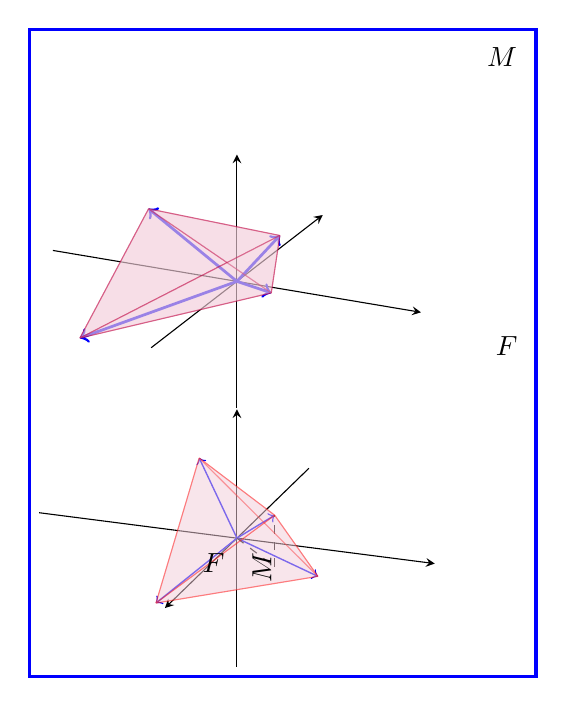
\begin{tikzpicture}

% PRACTICE PLOT
\matrix [row sep=0cm, column sep=0.5cm,draw=blue,very thick, style={align=center}] (my matrix) at (0,0)
{
\begin{axis}[
    axis lines=center,
    xlabel={$F$},
    ylabel={$M$},
    ymin=-10, ymax=10, ytick={0}, ylabel near ticks,
    xmin=-6, xmax=6, xtick={0}, xticklabel=$\pgfmathprintnumber{\tick}^\circ$, xlabel near ticks, 
    zmin=-10, zmax=10, ztick={0},
    xlabel style={at=(current axis.right of origin), anchor=north}, ylabel style={at=(current axis.above origin), anchor=east, rotate=-90},
    scale=1,
    anchor=center,
]
    \addplot3[->, line width=1pt, blue] coordinates {(0,0,0) (-4,4,2)};
    \addplot3[->, line width=1pt, blue] coordinates {(0,0,0) (-4,-4,-4)};
    \addplot3[->, line width=1pt, blue] coordinates {(0,0,0) (0,5,1)};
    \addplot3[->, line width=1pt, blue] coordinates {(0,0,0) (0,4,-3)};
    \addplot3[patch, opacity=0.4, fill=purple!20, faceted color=purple, patch type=triangle] 
        coordinates {
                    (-4,4,2) (-4,-4,-4) (0,5,1)
                    (-4,-4,-4) (0,5,1) (0,4,-3)
                    (0,5,1) (0,4,-3) (-4,4,2)
                    (0,4,-3) (-4,4,2) (-4,-4,-4)
                    };

\end{axis};
\\
% PRACTICE PLOT #2
\begin{axis}[
    view={110}{30},
    axis lines=center,
    % axis equal image,
    xlabel={$F$},
    ylabel={$M$},
    ymin=-10, ymax=10, ytick={0}, ylabel near ticks,
    xmin=-10, xmax=10, xtick={0}, xticklabel=$\pgfmathprintnumber{\tick}^\circ$, xlabel near ticks, 
    zmin=-10, zmax=10, ztick={0},
    % xlabel style={at=(current axis.right of origin), anchor=north}, ylabel style={at=(current axis.above origin), anchor=east, rotate=-90},
    scale=1,
    anchor=center,
    ]
    \def\pta{(3,3,4)}
    \def\ptb{(-3,-3,4)}
    \def\ptc{(3,-3,-4)}
    \def\ptd{(-3,3,-4)}
    \addplot3[->, line width=0.5pt, blue] coordinates {(0,0,0) (3,3,4)};
    \addplot3[->, line width=0.5pt, blue] coordinates {(0,0,0) (-3,-3,4)};
    \addplot3[->, line width=0.5pt, blue] coordinates {(0,0,0) (3,-3,-4)};
    \addplot3[->, line width=0.5pt, blue] coordinates {(0,0,0) (-3,3,-4)};
    % connector lines for perspective
    \addplot3[dashed] coordinates {(0,0,0) (3,3,0)};
    \addplot3[dashed] coordinates {(3,3,0) (3,3,4)}; 
    % faces of shape
    \addplot3[patch, opacity=0.3, fill=purple!20, faceted color=red, patch type=triangle] 
        coordinates {
                    \pta \ptb \ptc
                    \ptb \ptc \ptd
                    \ptc \ptd \pta
                    \ptd \pta \ptb
                    };
\end{axis};
\\
};
\end{tikzpicture}

    \caption{Caption}
    \label{fig:torque3d}
\end{figure}